\documentclass{beamer}
\usepackage{tikz}
\usepackage{fp}
\def \step{0.5}
% define the bounding box
\def \boundb{(-4,-2.5) rectangle (4,2.5)}
\def \band{[step=0.5cm](-4,-0.5) grid (4,0)}
\def \triangle{(0,0.25) -- (0.5,0.25) -- (0.25,0) -- cycle}
\def \state{(0,0.25) rectangle (0.5,0.75)}
\begin{document}
\begin{frame}
\frametitle{Turingmaschine}
\begin{center}
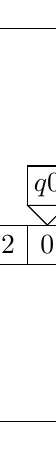
\begin{tikzpicture}[trim left=0,trim right=0] 
\draw \boundb; 
\clip \boundb; 
\draw \band; 
\draw \triangle;
\draw \state;
\node at (0.25,0.5) {{$q0$}};
\node at (-3,2) {Steps: {1}};
\def \start  {0.25}
\FPeval{start}{start-step*2}
\foreach \bit in {2,2,0,0,0,0,0,0,0,0,0,0,0,0,0,1,0,2,2}{
\node at (\start,-0.25) {\bit};
\FPeval{start}{start+step}
\xdef\start{\start}% make \xb global
}
\end{tikzpicture}
\end{center}
\end{frame}
\begin{frame}
\frametitle{Turingmaschine}
\begin{center}
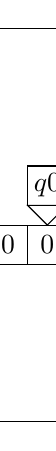
\begin{tikzpicture}[trim left=0,trim right=0] 
\draw \boundb; 
\clip \boundb; 
\draw \band; 
\draw \triangle;
\draw \state;
\node at (0.25,0.5) {{$q0$}};
\node at (-3,2) {Steps: {2}};
\def \start  {0.25}
\FPeval{start}{start-step*3}
\foreach \bit in {2,2,0,0,0,0,0,0,0,0,0,0,0,0,0,1,0,2,2}{
\node at (\start,-0.25) {\bit};
\FPeval{start}{start+step}
\xdef\start{\start}% make \xb global
}
\end{tikzpicture}
\end{center}
\end{frame}
\begin{frame}
\frametitle{Turingmaschine}
\begin{center}
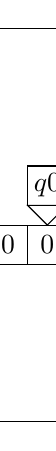
\begin{tikzpicture}[trim left=0,trim right=0] 
\draw \boundb; 
\clip \boundb; 
\draw \band; 
\draw \triangle;
\draw \state;
\node at (0.25,0.5) {{$q0$}};
\node at (-3,2) {Steps: {3}};
\def \start  {0.25}
\FPeval{start}{start-step*4}
\foreach \bit in {2,2,0,0,0,0,0,0,0,0,0,0,0,0,0,1,0,2,2}{
\node at (\start,-0.25) {\bit};
\FPeval{start}{start+step}
\xdef\start{\start}% make \xb global
}
\end{tikzpicture}
\end{center}
\end{frame}
\begin{frame}
\frametitle{Turingmaschine}
\begin{center}
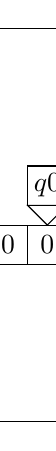
\begin{tikzpicture}[trim left=0,trim right=0] 
\draw \boundb; 
\clip \boundb; 
\draw \band; 
\draw \triangle;
\draw \state;
\node at (0.25,0.5) {{$q0$}};
\node at (-3,2) {Steps: {4}};
\def \start  {0.25}
\FPeval{start}{start-step*5}
\foreach \bit in {2,2,0,0,0,0,0,0,0,0,0,0,0,0,0,1,0,2,2}{
\node at (\start,-0.25) {\bit};
\FPeval{start}{start+step}
\xdef\start{\start}% make \xb global
}
\end{tikzpicture}
\end{center}
\end{frame}
\begin{frame}
\frametitle{Turingmaschine}
\begin{center}
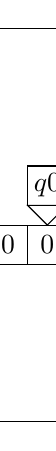
\begin{tikzpicture}[trim left=0,trim right=0] 
\draw \boundb; 
\clip \boundb; 
\draw \band; 
\draw \triangle;
\draw \state;
\node at (0.25,0.5) {{$q0$}};
\node at (-3,2) {Steps: {5}};
\def \start  {0.25}
\FPeval{start}{start-step*6}
\foreach \bit in {2,2,0,0,0,0,0,0,0,0,0,0,0,0,0,1,0,2,2}{
\node at (\start,-0.25) {\bit};
\FPeval{start}{start+step}
\xdef\start{\start}% make \xb global
}
\end{tikzpicture}
\end{center}
\end{frame}
\begin{frame}
\frametitle{Turingmaschine}
\begin{center}
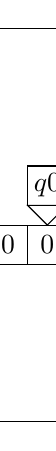
\begin{tikzpicture}[trim left=0,trim right=0] 
\draw \boundb; 
\clip \boundb; 
\draw \band; 
\draw \triangle;
\draw \state;
\node at (0.25,0.5) {{$q0$}};
\node at (-3,2) {Steps: {6}};
\def \start  {0.25}
\FPeval{start}{start-step*7}
\foreach \bit in {2,2,0,0,0,0,0,0,0,0,0,0,0,0,0,1,0,2,2}{
\node at (\start,-0.25) {\bit};
\FPeval{start}{start+step}
\xdef\start{\start}% make \xb global
}
\end{tikzpicture}
\end{center}
\end{frame}
\begin{frame}
\frametitle{Turingmaschine}
\begin{center}
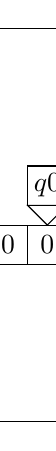
\begin{tikzpicture}[trim left=0,trim right=0] 
\draw \boundb; 
\clip \boundb; 
\draw \band; 
\draw \triangle;
\draw \state;
\node at (0.25,0.5) {{$q0$}};
\node at (-3,2) {Steps: {7}};
\def \start  {0.25}
\FPeval{start}{start-step*8}
\foreach \bit in {2,2,0,0,0,0,0,0,0,0,0,0,0,0,0,1,0,2,2}{
\node at (\start,-0.25) {\bit};
\FPeval{start}{start+step}
\xdef\start{\start}% make \xb global
}
\end{tikzpicture}
\end{center}
\end{frame}
\begin{frame}
\frametitle{Turingmaschine}
\begin{center}
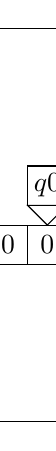
\begin{tikzpicture}[trim left=0,trim right=0] 
\draw \boundb; 
\clip \boundb; 
\draw \band; 
\draw \triangle;
\draw \state;
\node at (0.25,0.5) {{$q0$}};
\node at (-3,2) {Steps: {8}};
\def \start  {0.25}
\FPeval{start}{start-step*9}
\foreach \bit in {2,2,0,0,0,0,0,0,0,0,0,0,0,0,0,1,0,2,2}{
\node at (\start,-0.25) {\bit};
\FPeval{start}{start+step}
\xdef\start{\start}% make \xb global
}
\end{tikzpicture}
\end{center}
\end{frame}
\begin{frame}
\frametitle{Turingmaschine}
\begin{center}
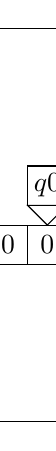
\begin{tikzpicture}[trim left=0,trim right=0] 
\draw \boundb; 
\clip \boundb; 
\draw \band; 
\draw \triangle;
\draw \state;
\node at (0.25,0.5) {{$q0$}};
\node at (-3,2) {Steps: {9}};
\def \start  {0.25}
\FPeval{start}{start-step*10}
\foreach \bit in {2,2,0,0,0,0,0,0,0,0,0,0,0,0,0,1,0,2,2}{
\node at (\start,-0.25) {\bit};
\FPeval{start}{start+step}
\xdef\start{\start}% make \xb global
}
\end{tikzpicture}
\end{center}
\end{frame}
\begin{frame}
\frametitle{Turingmaschine}
\begin{center}
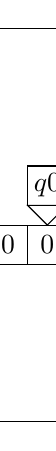
\begin{tikzpicture}[trim left=0,trim right=0] 
\draw \boundb; 
\clip \boundb; 
\draw \band; 
\draw \triangle;
\draw \state;
\node at (0.25,0.5) {{$q0$}};
\node at (-3,2) {Steps: {10}};
\def \start  {0.25}
\FPeval{start}{start-step*11}
\foreach \bit in {2,2,0,0,0,0,0,0,0,0,0,0,0,0,0,1,0,2,2}{
\node at (\start,-0.25) {\bit};
\FPeval{start}{start+step}
\xdef\start{\start}% make \xb global
}
\end{tikzpicture}
\end{center}
\end{frame}
\begin{frame}
\frametitle{Turingmaschine}
\begin{center}
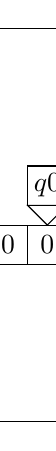
\begin{tikzpicture}[trim left=0,trim right=0] 
\draw \boundb; 
\clip \boundb; 
\draw \band; 
\draw \triangle;
\draw \state;
\node at (0.25,0.5) {{$q0$}};
\node at (-3,2) {Steps: {11}};
\def \start  {0.25}
\FPeval{start}{start-step*12}
\foreach \bit in {2,2,0,0,0,0,0,0,0,0,0,0,0,0,0,1,0,2,2}{
\node at (\start,-0.25) {\bit};
\FPeval{start}{start+step}
\xdef\start{\start}% make \xb global
}
\end{tikzpicture}
\end{center}
\end{frame}
\begin{frame}
\frametitle{Turingmaschine}
\begin{center}
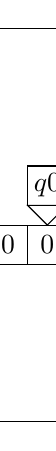
\begin{tikzpicture}[trim left=0,trim right=0] 
\draw \boundb; 
\clip \boundb; 
\draw \band; 
\draw \triangle;
\draw \state;
\node at (0.25,0.5) {{$q0$}};
\node at (-3,2) {Steps: {12}};
\def \start  {0.25}
\FPeval{start}{start-step*13}
\foreach \bit in {2,2,0,0,0,0,0,0,0,0,0,0,0,0,0,1,0,2,2}{
\node at (\start,-0.25) {\bit};
\FPeval{start}{start+step}
\xdef\start{\start}% make \xb global
}
\end{tikzpicture}
\end{center}
\end{frame}
\begin{frame}
\frametitle{Turingmaschine}
\begin{center}
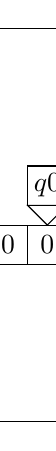
\begin{tikzpicture}[trim left=0,trim right=0] 
\draw \boundb; 
\clip \boundb; 
\draw \band; 
\draw \triangle;
\draw \state;
\node at (0.25,0.5) {{$q0$}};
\node at (-3,2) {Steps: {13}};
\def \start  {0.25}
\FPeval{start}{start-step*14}
\foreach \bit in {2,2,0,0,0,0,0,0,0,0,0,0,0,0,0,1,0,2,2}{
\node at (\start,-0.25) {\bit};
\FPeval{start}{start+step}
\xdef\start{\start}% make \xb global
}
\end{tikzpicture}
\end{center}
\end{frame}
\begin{frame}
\frametitle{Turingmaschine}
\begin{center}
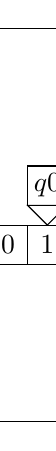
\begin{tikzpicture}[trim left=0,trim right=0] 
\draw \boundb; 
\clip \boundb; 
\draw \band; 
\draw \triangle;
\draw \state;
\node at (0.25,0.5) {{$q0$}};
\node at (-3,2) {Steps: {14}};
\def \start  {0.25}
\FPeval{start}{start-step*15}
\foreach \bit in {2,2,0,0,0,0,0,0,0,0,0,0,0,0,0,1,0,2,2}{
\node at (\start,-0.25) {\bit};
\FPeval{start}{start+step}
\xdef\start{\start}% make \xb global
}
\end{tikzpicture}
\end{center}
\end{frame}
\end{document}
